% XCircuit output "prototype.tex" for LaTeX input from prototype.ps
\def\putbox#1#2#3#4{\makebox[0in][l]{\makebox[#1][l]{}\raisebox{\baselineskip}[0in][0in]{\raisebox{#2}[0in][0in]{\scalebox{#3}{#4}}}}}
\def\rightbox#1{\makebox[0in][r]{#1}}
\def\centbox#1{\makebox[0in]{#1}}
\def\topbox#1{\raisebox{-0.60\baselineskip}[0in][0in]{#1}}
\def\midbox#1{\raisebox{-0.20\baselineskip}[0in][0in]{#1}}
   \scalebox{1}{
   \normalsize
   \parbox{4.86979in}{
   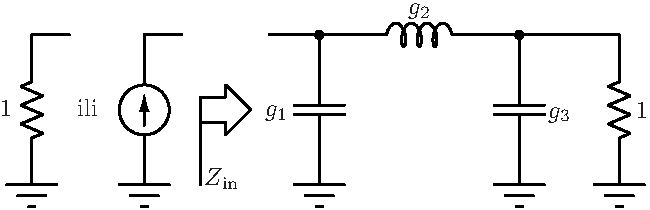
\includegraphics[scale=1]{prototype}\\
   % translate x=905 y=491 scale 0.38
   \putbox{1.80in}{0.06in}{1.20}{}%
   \putbox{3.10in}{2.75in}{1.20}{\centbox{$g_2$}}%
   \putbox{2.23in}{2.11in}{1.20}{\rightbox{\midbox{$g_1$}}}%
   \putbox{3.96in}{2.06in}{1.20}{$g_3$}%
   \putbox{4.55in}{2.06in}{1.20}{$1$}%
   \putbox{0.39in}{2.11in}{1.20}{\rightbox{\midbox{$1$}}}%
   \putbox{1.67in}{1.61in}{1.20}{\rotatebox{-360}{$Z_\mr{in}$}}%
   \putbox{0.89in}{2.11in}{1.20}{\centbox{\midbox{$\mr{ili}$}}}%
   } % close 'parbox'
   } % close 'scalebox'
   \vspace{-\baselineskip} % this is not necessary, but looks better
